\documentclass[border=0.2cm]{standalone}
\usepackage{tikz}
\usepackage{graphicx}
\usetikzlibrary{shapes.geometric} % for the hexagon
\usetikzlibrary{shapes} % for the hexagon

\begin{document}
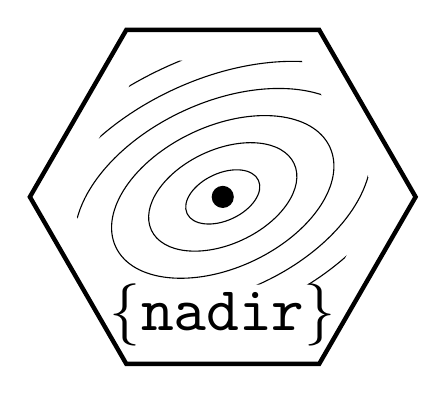
\begin{tikzpicture}[scale=2]
  % Create a clipping mask in the shape of a hexagon
  \begin{scope}
    % \clip (0,0) circle (3cm); % node [regular polygon, regular polygon sides = 6, fill = blue, inner sep=3cm] {blah};
    % \clip (-.952,-.3)--++(-:5cm)--++(75:4.5)--++(150:2cm)--++(200:3.5)--cycle;
    \clip ( {cos(60*1)} , {sin(60*1)} )
    -- ( {cos(60*2)} , {sin(60*2)} )
    -- ( {cos(60*3)} , {sin(60*3)} )
    -- ( {cos(60*4)} , {sin(60*4)} )
    -- ( {cos(60*5)} , {sin(60*5)} )
    -- ( {cos(60*6)} , {sin(60*6)} )
    -- cycle;
    
    % Draw multiple concentric ellipses inside the hexagon
    \foreach \r in {0.25, 0.5, ..., 3.5} {
      \draw[black] (0,0) ellipse [x radius=\r cm, rotate = 25, y radius=0.6*\r cm];
    }
    
    % Mark the central point with a filled circle
    \fill (0,0) circle (2pt);
  \end{scope}
  
  % Optionally, draw the hexagon outline to emphasize the mask
  \draw[black, thick] (0,0) node[regular polygon, regular polygon sides=6, inner sep = 1.5cm] {};
  \node[ultra thick, regular polygon, draw, regular polygon sides = 6, inner sep=1.5cm] (p) at (0, 0) {};
  
  % Add text at the bottom of the figure
  % \fill[draw=white,color=white] (-.75,-.75) rectangle (.75,-.56);
  \fill[draw=white,color=white] (-.75,-.56) -- (.75,-.56) -- (.45, -.95) -- (-.45, -.95) -- cycle;
  \node [scale=2.25, color=black] at (0,-.75) {\texttt{\{nadir\}}};
\end{tikzpicture}
\end{document}

